\documentclass[conference,final,a4paper,twocolumn,9pt]{IEEEtran}

\usepackage{cmap}
\usepackage[utf8x]{inputenc}
\usepackage[T1]{fontenc}

\usepackage{lmodern}

\usepackage{mathtools}
\usepackage{amssymb}

\usepackage[USenglish]{babel}

\usepackage{array}
\usepackage{amsthm}
\usepackage{amsfonts}
\usepackage{mathtools}
\usepackage{makeidx}
\usepackage[pdftex]{graphicx}
\usepackage{url}
\usepackage{epigraph}
\usepackage{hyperref}
\usepackage{natbib}

\ifCLASSINFOpdf
\usepackage[pdftex]{graphicx}
\DeclareGraphicsExtensions{.pdf,.jpeg,.png}
\else
\usepackage[dvips]{graphicx}
\DeclareGraphicsExtensions{.eps}
\fi

\usepackage{amsmath}
\usepackage{algorithmic}
\usepackage{url}

\usepackage{tikz, pgfplots}
\usepackage{tikz-qtree}

\usetikzlibrary{patterns}

\begin{document}
\title{RobOptim: an Optimization Framework for Robotics}

\author{\IEEEauthorblockN{Thomas Moulard}
\IEEEauthorblockA{FIXME}
\and
\IEEEauthorblockN{Florent Lamiraux}
\IEEEauthorblockA{FIXME}
\and
\IEEEauthorblockN{Karim Bouyarmane}
\IEEEauthorblockA{FIXME}
\and
\IEEEauthorblockN{Eiichi Yoshida}
\IEEEauthorblockA{FIXME}}

\maketitle

\begin{abstract}
\boldmath
The abstract goes here.
\end{abstract}

\IEEEpeerreviewmaketitle

\section{Introduction}\label{sec:introduction}


Over the past years, numerical optimization proved itself particulaly
suited for various robotics use such as posture or trajectory
optimization, robot control and more. These applications yield both
linear and non-linear optimizations problems with equalities and
inequalities constraints. Robot control also relies on other types of
optimization problems such as quadrating programming. As these
algorithms must run in real-time, it leads to strong constraints on
the implementation efficiency. The design and implementation of a
solver is tedious and error-prone. Avoiding numerical precision
issues, assuring that the algorithm behaves properly in all cases and
reports correctly the errors it may encounter is challenging, in
particular for roboticians which are not experts in optimization
techniques. Among available optimization toolboxes, the Matlab
Optimization Toolbox[CITE], the Open Optimization library, OPT++,
IPOPT, SciPy and the GSL (Gnu Scientific Library) all provides some
optimization algorithms. Unfortunately, these libraries suffer from
several drawbacks: difficult to use, no support for advanced
algorithms such as support for constrained optimization, efficiency
issues, etc. They also all lack a unified model expressing
optimization problems.


RobOptim solves these limitations by introducing a model allowing to
express any continuous optimization problem, constrained or not. Its
design was focused on providing an easy to use C++ set of libraries, a
safe and efficient framework which can be used to prototype robotics
applications. The RobOptim computational model will be first
introduced in~\autoref{sec:roboptim} and different applications will
be detailed in~\autoref{sec:application}. In particular, an extension
of RobOptim for a particular type of problem has been realized
recently, demonstrating the ability of RobOptim to support a variety
of problems. The conclusion will detail feedback from current users of
RobOptim and present the roadmap for the next developments.


\section{RobOptim overview}\label{sec:roboptim}


RobOptim is a set of open-source C++ libraries licensed under the LGPL
license. Code source, documentation and examples are available on the
project webpage: \mbox{\url{http://www.roboptim.net/}}.


The RobOptim framework is divided into three parts. The core layer
provides a computation model expressive enough to model different
types of optimization problems. The solver layer gathers different
optimization algorithms which are.


\subsection{Mathematical functions representation}


Continuous optimization problems can be defined as follow:

\begin{equation}\label{eq:optimization}
  \min_{\mathbf{x} \in \mathbb{R}^n} f(\mathbf{x}) \text{ under the constraint } \mathbf{x} \in \mathbf{X}
\end{equation}

where $f : \mathbb{R}^n \mapsto \mathbb{R}$ is the cost function and
$\mathbf{X} \subset \mathbb{R}^n$ is the space of the admissible
solutions. This space is usually defined by a set of inequality and
equality constraints:

\begin{equation}
  \mathbf{X} \equiv \left\{
  \begin{array}{l l}
    c_i (x) = 0    & \quad i \in \xi \\
    c_j (x) \leq 0 & \quad j \in \nu \\
  \end{array} \right.
\end{equation}

$c_i$, $c_j$ are respectively the set of equality and inequality
constraints. $i$ and $j$ are the indices identifying the constraints.

The mathematical functions $f$ and $c_k$, $k \in \xi \cup \nu$ must
provide a way to evaluate their result at any point they are
defined. Their associated gradient and hessian may also be
provided. To finish, each of these function may have a particular
structure that can help the resolution. The goal of the RobOptim core
layer is to express these features through the C++ typing rules.


Depending on the solving algorithm, it may be necessary to obtain the
jacobian and in some cases even the hessian of the used
functions. Hence, a function which provides the maximum information
about itself will be usable with a larger proportion of solvers.

\begin{figure}
  \begin{center}
    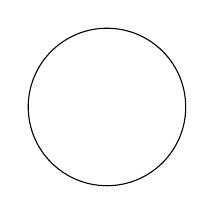
\begin{tikzpicture}
      \draw (0,0) circle (1) ;
    \end{tikzpicture}
  \end{center}
  \caption{Sets representing the different kind of functions that
    RobOptim can model out-of-the-box.}\label{fig:functions}
\end{figure}

In RobOptim, each mathematical function is represented by a different
C++ class. All of these types then inherit from the abstract kind of
mathematical functions they represent. The following kind of
mathematical functions are bundled with RobOptim core: function that
can evaluate itself (Function type), function evaluate itself and its
gradient (DifferentiableFunction), function that can evaluate itself,
its gradient and its hessian (TwiceDifferentiableFunction), etc.  Let
'A <: B' denote the relationship ``type B is a subtype (subclass) of
A'' or ``B inherits from A''. Then a partial order can be defined
where: Function <: DifferentiableFunction <:
TwiceDifferentiableFunction. It can also be understood through sets
as illustrated by~\autoref{fig:functions}.


\subsection{Optimization problem definition and problem resolution}


Once function cost and all constraints functions have been
implemented, an optimization problem has to be built. RobOptim core
provides a meta-class Problem parametrized by two parameters $F$ and
$C_L$. $F$ is the type of the cost function and $C_L$ is the list of
the constraints types. A non-linear problem with constraints then has
the following type:


\texttt{Problem<DerivableFunction, vector<LinearFunction, DerivableFunction > >}


The constraints can be either linear or non-linear. With this
constraint type definition, the constraints will be divided into two
categories which will help the solver to perform efficiently.

Additionally, bounds can be set on the optimization variables and a
starting point for the optimization process can be set. When the
constraints are added to the problem, each constraint is associated
with an interval. If this interval is reduced to a point, the
constraint is an equality constraint. At each time of the problem
construction at both compile time and run-time, RobOptim checks that
only valid problem are built. For instance if one add a constraint of
type $T$ then RobOptim checks at compile time that the constraint is a
subtype of $T$.


Once the problem is defined, a solver need to be instantiated that
will solve the problem. Each solver is parametrized by the same
variables than an optimization problem. Therefore the solver
$S<P_1,C_{L1}>$ can solve the problem $P<P_2,C_{L2}>$ if the following
relation is true:


\begin{equation}
  P_1 <: P_2 \wedge \forall i, C_{L1}(i) <: C_{L2}(i)
\end{equation}


Basically, the problem can be solved if all types provide enough or
more information than necessary. For instance if gradient are
required, the function may also provide hessian computation but if
gradient are lacking the compile time assertions will fail and prevent
the user from building an invalid optimization problem.

By separating problem expression from solver, dynamic changes of the
solving algorithm are possible. Each solver is bundled as a plug-in
which is loaded at run-time. An interest is to let the user change its
problem complexity during its design process freely. Other frameworks
would require a different API depending on the kind of optimization at
hand, here the changes are minimal. One may choose to use a more
powerful than required solver at first and then refince their choice
or implement later a new plug-in providing the best algorithm for one
particular application. These features are provided through
meta-programming techniques and come with a near zero
cost\footnote{RobOptim core do not realize copy so the additional
  runtime cost is only due to calls to virtual functions.} at runtime
and are unique to RobOptim.

\subsection{Costs and constraints toolbox}


Unlike others


\section{Applications and case study}\label{sec:application}

\subsection{Step planning for humanoid robots}
\subsection{Posture optimization for humanoid robots}
\subsection{Extending the framework: least square optimization}

\section{Conclusion}\label{sec:conclusion}

\section*{Acknowledgments}\label{sec:acknowledgments}

\end{document}
